\chapter{ПРАКТИЧЕСКАЯ РАБОТА № 5 <<ДИАГРАММА СИСТЕМНОГО КОНТЕКСТА И ДИАГРАММА ВАРИАНТОВ ИСПОЛЬЗОВАНИЯ>>}

\section{Цель работы}

Цель работы: целью данной практической работы является ознакомление с формальной семантикой UML-диаграммы вариантов использования и применением диаграмм при проектировании архитектуры программного обеспечения, а также выявление особенностей их использования на практике.

\section{Теоретическое введение}

Использование UML, при правильной организации процесса моделирования, позволяет раскрыть особенности архитектуры разрабатываемого ПО с требуемым уровнем детализации для каждого из участников проекта. При разработке архитектур на ранних этапах полезно определить только те характеристики, которые на этом этапе будут с требуемой точностью определять основные концептуальные особенности разрабатываемой программной системы, тем самым, четко определив концептуальные границы разрабатываемого ПО, что позволит определить ту отправную точку, которая будет показывать, как программная система по своему объему вписывается в окружающий мир, а также представит общий вид программной системы. Для этих целей можно использовать, так называемую, системную контекстную диаграмму.

Диаграмма вариантов использования представляет проектируемую систему в виде множества сущностей или актёров, которые взаимодействуют с этой системой посредством вариантов использования. Варианты использования описывают поведение моделируемой системы при различных условиях и воздействиях на неё со стороны заинтересованных лиц, которых называют актёрами. Как было отмечено выше, основной целью диаграмм вариантов использования является охват всех функций системного уровня, которые будут использовать эту разрабатываемую программную систему.

Каждый вариант использования должен относиться к конкретному классу пользователей системы, которые представлены актёром. Актёр может представлять любую сущность, например пользователь системы, сторонняя информационная система, интеллектуальный агент и т.д. При этом один пользователь может входить в разные классы одновременно. В качестве примера можно привести тот случай, когда администратор системы, обладающий правами администратора, может являться и пользователем системы, права которого ограничены.
Диаграмма вариантов использования описывает отношения между участниками и различными вариантами использования, которые в нотациях UML называются ассоциациями. Отношения ассоциации не имеют направленности, а представляют собой лишь линии между актёрами и вариантами использования.

\subsection{Диаграмма ассоциации}

Диаграмма вариантов использования описывает отношения между участниками и различными вариантами использования, которые в нотациях UML называются ассоциациями. Отношения ассоциации не имеют направленности, а представляют собой лишь линии между актёрами и вариантами использования.

\subsection{Диаграмма отношения обобщения}

Помимо отношений ассоциации актёры, а также варианты использования могут быть связаны отношениями обобщения. Отношения обобщения всегда направлены. 

Отношение обобщения от актёра - администратора системы к актёру --- владельца системы устанавливает то обстоятельство, что роли администратора имеют все функции и свойства присущие владельцам файлов, которые, в частности, позволяют им удалять любые файлы, которые они захотят.

\subsection{Отношения включения}

Вариант использования может зависеть от другого варианта, то есть поведение одного варианта может быть составной частью поведения другого варианта. Например, вариант использования «удалить файл» в обязательном порядке будет включать в себя вариант использования «проверить права доступа». Направление пунктирной линии со стрелкой и надписью «INCLUDE» идёт от основного варианта использования к включённому варианту использования.

\subsection{Отношения расширения}

Вариант использования может, при определённых обстоятельствах, вызывать другой вариант использования, например для предоставления некоторой альтернативы. В таком случае говорят, что данная зависимость является расширенной. Направление пунктирной линии со стрелкой и с надписью «EXTEND» идёт от расширения к расширенному варианту использования. 

\section{Цель}

Используя средства UML, необходимо разработать диаграмму использования для системы бронирования билетов на автовокзале. Разрабатываемая система должна обеспечивать возможность покупки билетов через электронный киоск при предъявлении паспорта (паспорт сканируется при начале работы с киоском). Актёры - пассажир со следующими атрибутами: ФИО, адрес регистрации, номер и серия паспорта, город прибытия. Операции: бронировать билет.

\section{Выполнение работы}

\begin{figure}[h!]
        \centering
        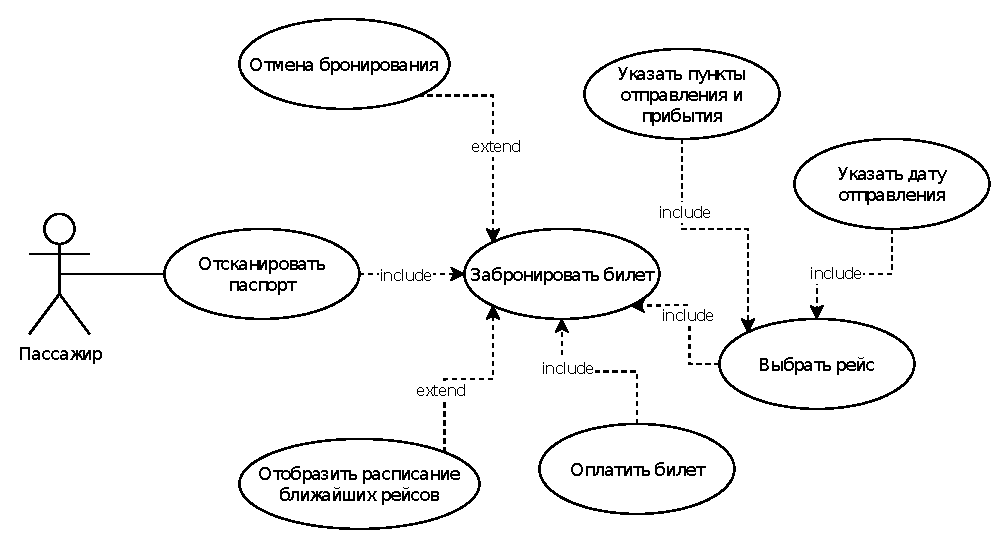
\includegraphics[width=\textwidth]{images/5/uml.eps}
        \caption{Организационная структура объекта}
	\label{uml}
\end{figure}

В ходе выполнения работы была реализована диаграмма \ref{uml}. 

Опишем элементы системы.

\subsection{Актор}

Актор --- пассажир (человек) с ФИО, адресом регистрации, номером и серией паспорта, городом прибытия.
Отношения ассоциации не имеют направленности, а представляют собой лишь линии между актёрами и вариантом использования --- элементом <<Отсканировать паспорт>>.

\subsection{Отсканировать паспорт}

Точка входа в систему. 

От неё исходит отношение включения к варианту использования <<Забронировать билет>>.

\subsection{Забронировать билет}
В нее входят варианты использования с отношением включения <<Оплатить билет>> и <<Выбрать рейс>>. В нее входят варианты использования с отношением расширения <<Отобразить расписание ближайших рейсов>> и <<Отмена бронирования>>.

\subsection{Выбрать рейс}

Третья опорная точка системы, в нее включены варианты использования с отношением включения <<Указать пункты отправления и прибытия>>, <<Указать дату отправления>>.

\section{Вывод}

Ознакомились с формальной семантикой UML-диаграммы вариантов использования и применением диаграмм при проектировании архитектуры программного обеспечения, а также выявлением особенностей их использования на практике.
